\documentclass{beamer}

% ************* Preamble *************************** 
% Language setting
% Replace `english' with e.g. `spanish' to change the document language
\usepackage[english]{babel}

% Useful packages
\usepackage{amsmath}
% \usepackage{graphicx} %already loaded by beamer document class
\graphicspath{{../figures/}}
% \usepackage{hyperref} %already loaded by beamer document class
\usepackage{blindtext} % to generate 2 pages of text
\usepackage{booktabs} % nicer tables w/ mid, top, bottom rules
\usepackage{dcolumn} % should align decimals in tables
\newcolumntype{d}[1]{D{.}{.}{#1}} % command for dcolumn, use d{2} instead of l,
% or c in tabular column specifier

 

% Dont use caption/ subcaption in beamer, use columns instead.
\usepackage[compatibility=false]{caption} % for subfigures (panels)
\usepackage{subcaption} % for subfigures (panels)
% \setbeamertemplate{caption}[numbered] %to get figures to be numbered in beamer class

% Biblatex (options taken from Igors Github, is it equal to JoF style?)
\usepackage[
    backend=biber,
    style=bwl-FU,
    url=false,
    doi=false,
    eprint=false
]{biblatex}
% \addbibresource{references.bib}


% Title
\title{DTFF Final Project Presentation}

% \author[test]{Egemen Erdogdu\thanks{Egemen Erdogdu, University of Zurich, Rämistrasse 71, 8006 Zürich} \and Jonas Schmidiger\thanks{Jonas Schmidiger, University of Zurich, Rämistrasse 71, 8006 Zürich} \and Mathias Ruoss\thanks{Mathias Ruoss, University of Zurich, Rämistrasse 71, 8006 Zürich}}
\author[E. Erdogdu, J. Schmidiger, M. Ruoss] % (optional, for multiple authors)
{E. Erdogdu\inst{1} \and J. Schmidiger\inst{2} \and M. Ruoss\inst{3}}

\institute[UZH] % (optional)
{
  \inst{1}%
  Faculty of Banking and Finance\\
  Very Famous University
  \and
  \inst{2}%
  Faculty of Banking and Finance\\
  Very Famous University
  \and
  \inst{3}%
  Faculty of Banking and Finance\\
  Very Famous University
}
\date{\today}

\AtBeginSection[ ]
{
\begin{frame}{Outline}
    \tableofcontents[currentsection]
\end{frame}
}

\usetheme{Madrid}
% \usecolortheme{orchid}

% ***********************************************
\begin{document}

\frame{\titlepage}

\begin{frame}{Outline}
  \tableofcontents
\end{frame}

\section{Introduction}
\begin{frame}{Introduction}
  \begin{itemize}
    \item Is there a simple trading strategy that outperforms Buy\&Hold by 10x?
    \item As we found out, yes!
    \item To sum up: there was never a easier strategy than that one.
  \end{itemize}
\end{frame}

\section{Background}
\begin{frame}
    \frametitle{A theorem}
    \framesubtitle{Frame subtitle}
    \begin{theorem}
        $a^2 + b^2 = c^2$
    \end{theorem}
\end{frame}

\begin{frame}
    \frametitle{Some equations}
    \framesubtitle{Frame subtitle}
    % \begin{equation}
        \begin{align}
            y + x = 3\\
            y + 3 + 4 = 10\\
            y + \mathbf{x} + Z = 3
        \end{align}
    % \end{equation}
\end{frame}

\section{Dataset}
% Exercise 1 of lecture 6-Visualization
\begin{frame}
  \frametitle{A table with the package \texttt{dcolumn}}
\begin{table}[]
  \resizebox{\textwidth}{!}{
  \begin{tabular}{@{}ld{3}d{3}d{3}d{3}d{3}d{3}@{}}
  \toprule
  \multicolumn{1}{l}{Stock}       & \multicolumn{1}{c}{FB} & \multicolumn{1}{c}{AMZN} & \multicolumn{1}{c}{AAPL} & \multicolumn{1}{c}{NFLX} & \multicolumn{1}{c}{GOOGL} &  \\ \midrule
  Panel A: Descriptive statistics &        &        &        &        &        &  \\ \midrule
  Mean                            & 0.083  & 0.065  & 0.112  & 0.051  & 0.091  &  \\
  Variance                        & 0.041  & 0.030  & 0.044  & 0.061  & 0.037  &  \\
  Median                          & 0.064  & 0.058  & 0.091  & 0.043  & 0.102  &  \\
  Maximum                         & 0.053  & 0.064  & 0.078  & 0.043  & 0.062  &  \\
  Minimum                         & -0.211 & -0.181 & -0.195 & -0.203 & -0.081 &  \\
  Jarque Bera                     & 95.35   & 81.54   & 49.27   & 40.58   & 0.58   &  \\ \bottomrule
  \end{tabular}
  }
  \end{table}
\end{frame}


\begin{frame}
    \frametitle{A figure with two panels}
    \framesubtitle{A Subtitle}
    \begin{figure}
    \centering
      \begin{subfigure}{0.45\textwidth}
        \centering
        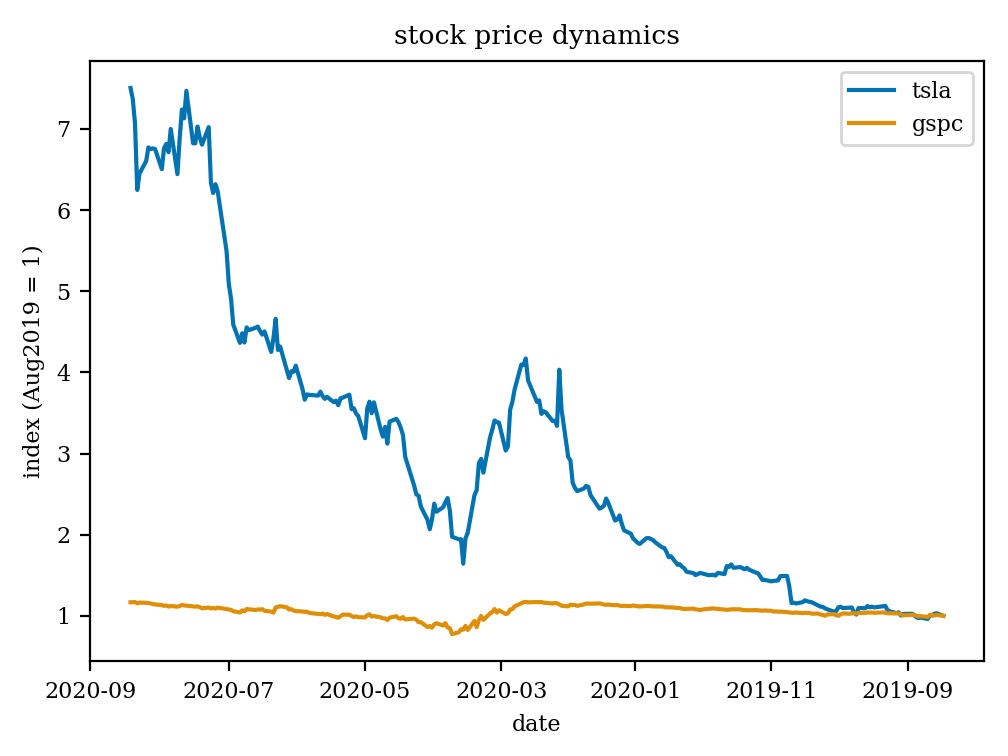
\includegraphics[width=\textwidth]{stock-index-weird-plot}
        \caption{First subfigure}
        \label{fig:a}
      \end{subfigure}\hfill
      \begin{subfigure}{0.45\textwidth}
        \centering
        % Figures taken from igors github
        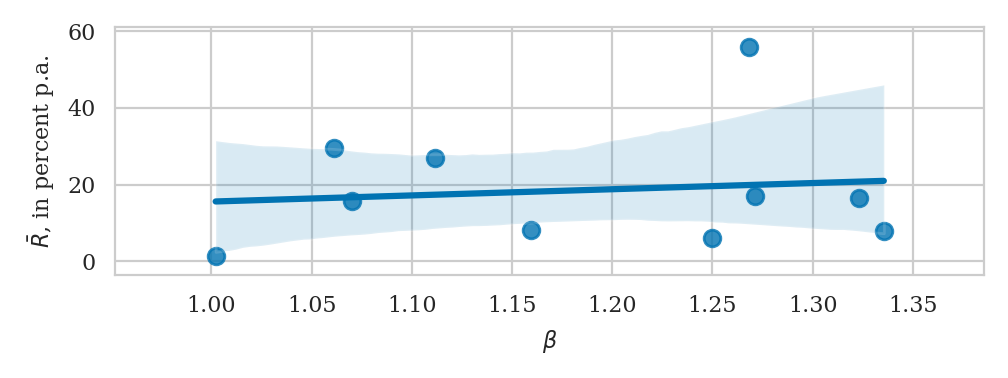
\includegraphics[width=\textwidth]{beta-vs-mu}
        \caption{Second subfigure}
        \label{fig:b}
      \end{subfigure}\\
    \caption{Two panels side by side}\label{fig:stock-beta-comparison}
    \end{figure}
\end{frame}

\begin{frame}
    \frametitle{Another figure with two panels aligned}
    \framesubtitle{Another subtitle}
    \begin{figure}[H]
        \centering
        \subcaptionbox{First subfigure}%
          [.45\linewidth]{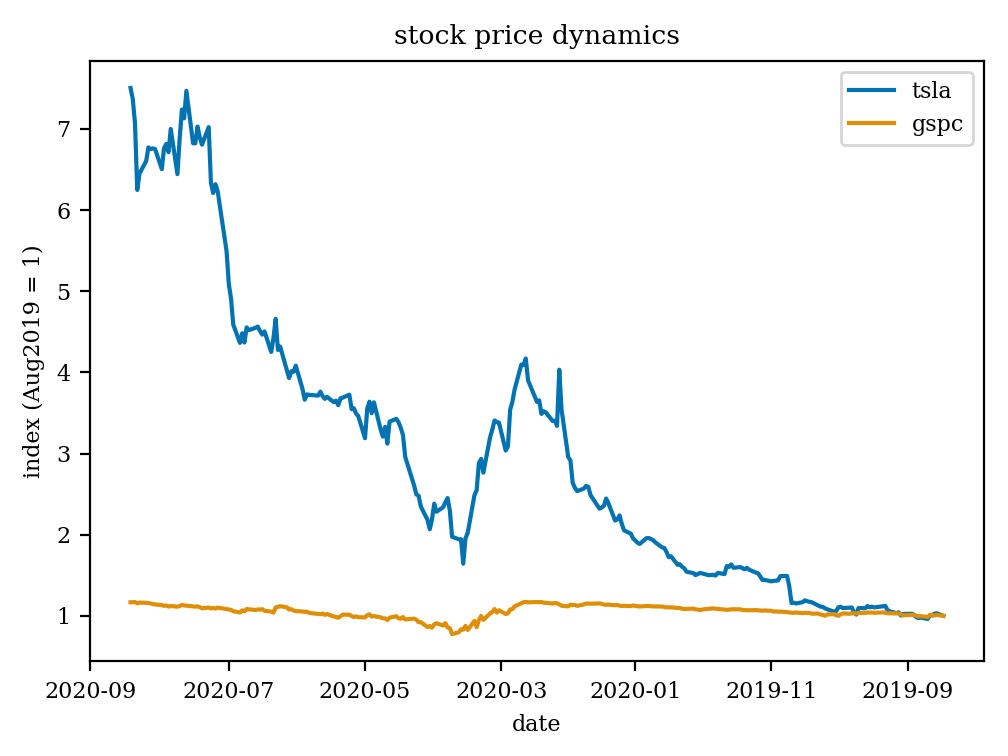
\includegraphics[height=3.5cm]{stock-index-weird-plot.png}}
        \subcaptionbox{Second subfigure}
          [.45\linewidth]{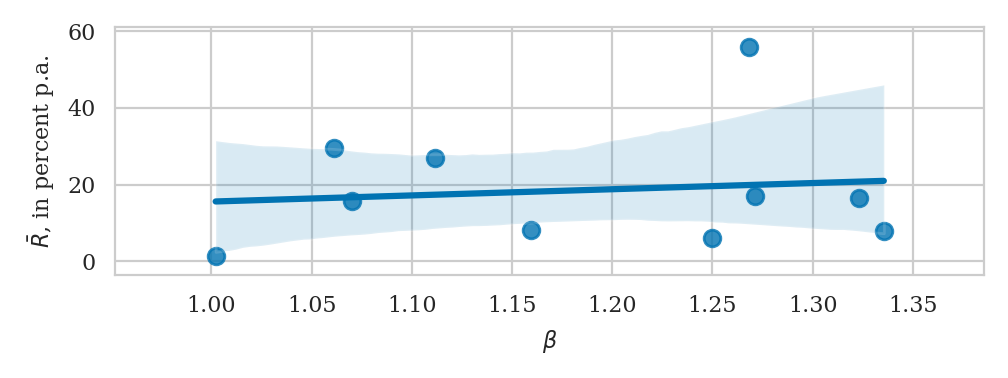
\includegraphics[height=2cm]{beta-vs-mu.png}}
    \caption{Two panels side by side}    
    \end{figure}        
\end{frame}

% Exercise 2, table as heatmap
\section{Results}
\begin{frame}
    \frametitle{A table as a heatmap}
    % \framesubtitle{Another subtitle}
    \begin{figure}[H]
      \centering
      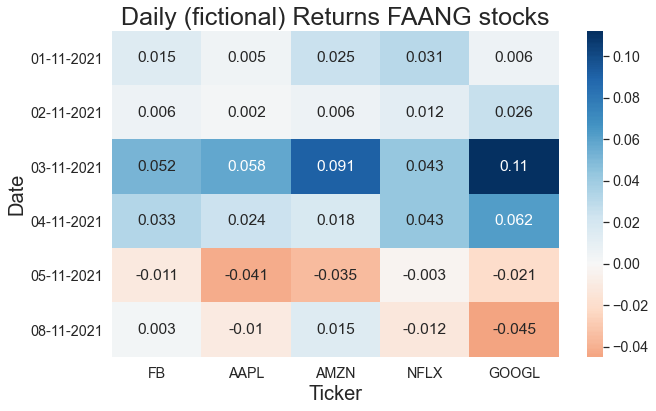
\includegraphics[width=\linewidth]{heatmap.png}
      % \caption{heatmap of returns}    
    \end{figure}        
\end{frame}


% Exercise 3, line plot with color friendly palette -> see code in "lineplot.py"
% we used the option palette="colorblind" in seaborn, a python package
\begin{frame}
  \frametitle{A table as a lineplot}
  % \framesubtitle{Another subtitle}
  \begin{figure}[H]
    \centering
    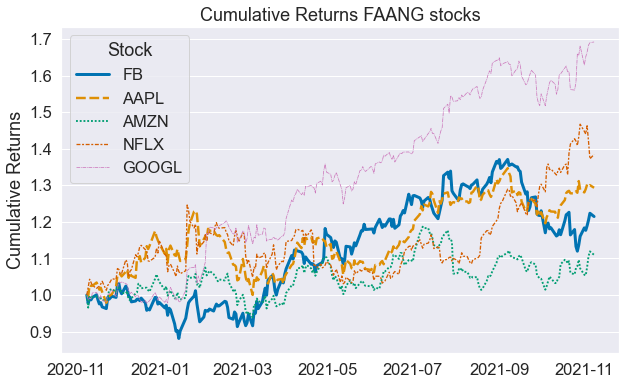
\includegraphics[width=\linewidth]{lineplot_beamer}
    % \caption{heatmap of returns}    
  \end{figure}        
\end{frame}

% Answer exercise 4:
% Grids could be pre-attentive, as the human brain learns spatial information
% from it. It also could be a learned pattern, e.g. through our school system, as we 
% learn how to read and write on sheets with horizontal and vertical grids.
\section{Conclusion}
\begin{frame}{Conclusion}
  \begin{itemize}
    \item New approach to construting a trading strategy that outperforms B\&H by 10x
    \item Could be used for all kinds of assets
    \item Further research should be done, as our study has limitations (high max. DD!)
  \end{itemize}
\end{frame}
\section*{References}

\end{document}